% 2007 年天津卷文科第 16 题：4 个相邻格子的横向长条（着色计数题配图）。
% 来源 PDF：source.pdf，SHA256 f4257944971547472f433b7da4dedb1dad9763fd284397f12daf6cf52c58283a
% 原页：source.pdf 第 1 页（A3 三栏）第 2 栏，书页码 415，图在第 16 题题干下方。
% 题面另要求「两端的格子的颜色也不同」，四格按环 C4 理解，与图形是否成环无关。
% 重绘依据：原图为透视「丝带」式画法——底边水平、四格等宽、分隔线竖直、顶边自左向右
%   平直上斜（左格高:格宽 ≈ 0.64，右格高:格宽 ≈ 1.2）。此处按原图同比重画，
%   格宽 1.5cm，左格高 0.96cm，右格高 1.79cm，中间各格顶高按直线内插。
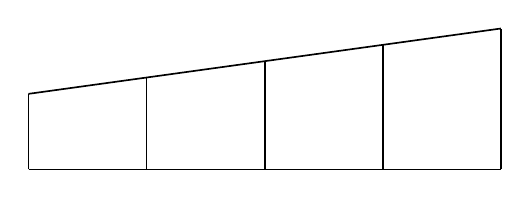
\begin{tikzpicture}[semithick]
  \draw (0,0) -- (6,0);
  \draw (0,0.96) -- (6,1.79);
  \draw (0,0) -- (0,0.96);
  \draw (1.5,0) -- (1.5,1.1675);
  \draw (3,0) -- (3,1.375);
  \draw (4.5,0) -- (4.5,1.5825);
  \draw (6,0) -- (6,1.79);
\end{tikzpicture}
